\documentclass[tikz,border=2pt,11pt]{standalone}
\usetikzlibrary{arrows.meta}
\usetikzlibrary{calc}
\usetikzlibrary{positioning}
\usepackage{amsmath}
\usepackage{amssymb}
\usepackage{tikz}
\newcommand{\F}{\mathbb F}
\newcommand{\St}{\operatorname{St}}
\newcommand{\E}{\operatorname{E}}
\newcommand{\eps}{\varepsilon}
\newcommand{\op}{\mathrm{op}}
\DeclareMathOperator{\im}{im}
\DeclareMathOperator{\diag}{diag}
\begin{document}
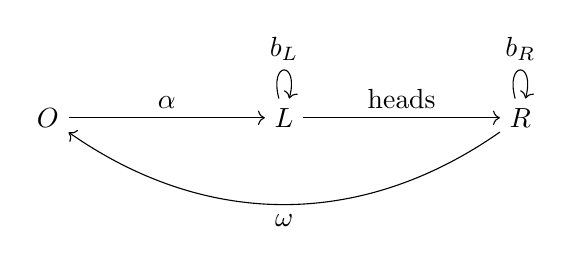
\begin{tikzpicture}[scale=1]
\node (O) at (0,0) {$O$};
\node (L) at (3,0) {$L$};
\node (R) at (6,0) {$R$};
\draw[->] (O) -- node[above] {$\alpha$} (L);
\draw[->] (L) -- node[above] {heads} (R);
\draw[->] (R) to[bend left=35] node[below] {$\omega$} (O);
\draw[->] (L) to[loop above] node[above] {$b_L$} (L);
\draw[->] (R) to[loop above] node[above] {$b_R$} (R);
\end{tikzpicture}
\end{document}
